\documentclass[]{article}
\usepackage{graphicx}
\graphicspath{{imagenes/}}
\usepackage[spanish]{babel}
\usepackage[a4paper, top=2.5cm, bottom=2.5cm, left=3cm, right=3cm]{geometry}
\usepackage[hidelinks]{hyperref}
\usepackage[T1]{fontenc}
\usepackage{listings}
\usepackage{xcolor}
\usepackage{float}
\usepackage{booktabs}
\usepackage{multirow}
\usepackage{amsmath}


% Configurar el color de los enlaces
\hypersetup{
    colorlinks=true, % Activa el color en los enlaces
    linkcolor=blue,  % Color para los enlaces internos (por ejemplo, tablas de contenido)
    citecolor=black,  % Color para las citas bibliográficas
    filecolor=blue,  % Color para enlaces a archivos
    urlcolor=blue    % Color para los enlaces a URLs
}


\definecolor{miverde}{rgb}{0,0.6,0}
\definecolor{miazul}{rgb}{0.5,0.5,1}
\lstdefinelanguage{cql}{
  morekeywords={SELECT, FROM, WHERE, INSERT, INTO, UPDATE, DELETE, CREATE, TABLE, PRIMARY, KEY, IF, EXISTS, NOT, NULL, AND, OR, SET, USE, VALUES, IN, ALLOW, FILTERING, AS}, % Palabras clave
    ndkeywords={COUNT, AVG},
    ndkeywordstyle=\color{miazul},
  sensitive=false, % Si las palabras clave distinguen mayúsculas de minúsculas
  morecomment=[l]--, % Comentarios de línea (prefijados con "--")
  morecomment=[s]{/*}{*/}, % Comentarios de bloque
  morestring=[b]', % Cadenas entre comillas simples
  morestring=[b]" % Cadenas entre comillas dobles
}


\lstdefinestyle{cql}{
    language=cql,
    backgroundcolor=\color{gray!2},     % Color de fondo
    basicstyle=\ttfamily,               % Tipo y tamaño de fuente
    keywordstyle=\color{blue}\bfseries, % Color para palabras clave
    stringstyle=\color{miverde},        % Color para cadenas
    commentstyle=\color{red},           % Color para comentarios
    showspaces=false,                   % No mostrar espacios
    showstringspaces=false,             % No mostrar espacios en las cadenas
    frame=single,                       % Poner un marco alrededor del código
    breaklines=true,                    % Romper las líneas largas
    captionpos=b,                       % Posición del caption
    tabsize=4,                          % Tamaño de las tabulaciones
    escapeinside={\%*}{*)},             % Para incluir código LaTeX en los listings
    morekeywords={self},                 % Palabras clave adicionales
    extendedchars=true,
    inputencoding=utf8
}

%title
\title{Práctica 1} 

\author{Adrián Ferández Galán, César López Mantecón y Manuel Gómez-Plana Rodríguez}

\begin{document}

\begin{titlepage}
    \centering
   
\includegraphics[width=0.9\textwidth]{uc3m.jpg} 
    {\Huge Universidad Carlos III\\
    
     \Large Arquitectura de Datos\\
     \vspace{0.5cm}
     Curso 2024-25}
    \vspace{2cm}

    {\Huge \textbf{Práctica 2} \par}
    \vspace{0.5cm}
    {\Large Migración de una base de datos a \texttt{Cassandra} \par}
    \vspace{8cm}

   \textbf{Ingeniería Informática, Cuarto curso}\\
    \vspace{0.2cm} 
    Adrián Fernández Galán       (NIA: 100472182, e-mail: 100472182@alumnos.uc3m.es)\\
    César López Mantecón         (NIA: 100472092, e-mail: 100472092@alumnos.uc3m.es)\\
    Manuel Gómez-Plana Rodríguez (NIA: 100472310, e-mail: 100472310@alumnos.uc3m.es)
    \vspace{0.5cm}

   
    \textbf{Prof .} Lourdes Moreno López\\
    
    \textbf{Grupo: } 81   
    
\end{titlepage}
\newpage

\renewcommand{\contentsname}{\centering Índice}

\hypersetup{linkcolor=black}
\tableofcontents
\hypersetup{linkcolor=blue}
\newpage

\section{Introducción}
\label{sec:introduccion}
En este documento se recoge el desarrollo de la práctica 2 de la asignatura
\textit{Arquitectura de Datos}. En esta práctica se tratará de completar una
migración de una base de datos desde \texttt{MongoDB} a \texttt{Cassandra}.
Además, se computarán nuevas tablas con el fin de permitir el análisis
estadístico, aprovechando las cualidades de \texttt{Cassandra} para el análisis
de datos gracias a su capacidad para la consulta masiva de datos de una misma
columna.

La metodología usada para el desarrollo de este proyecto ha sido la siguiente:
análisis de datos y casos de uso, realización del diseño lógico y físico
orientado a \texttt{Cassandra} e implementación de casos de uso en forma e
consulta. Adicionalmente se empleará la herramienta \texttt{PySpark} para
realizar el primer volcado de datos.

En el diseño de consultas se tratará de aprovechar al máximo las capacidades de
\texttt{Cassandra} en la lectura y escritura, dejando a la aplicación otra clase de
operaciones. De esta forma, ambos sistemas trabajarán en conjunto, garantizando
la eficiencia de la aplicación.


% =======
% Para la realización de esta práctica se busca realizar una migración de datos desde el gestor de bases de datos \textit{Mongodb} a \textit{Cassandra}, además de suplir una serie de casos de uso 
% 
% Esta práctica se basa en la migración de un sistema gestor de expedientes de sanciones que se encontraba en el gestor de bases de datos \textit{Mongodb} y se quiere mover a \textit{Cassandra}, además de implementar nuevos casos de uso. 
% Para ello se realizará un estudio de los datos almacenados en \textit{mongodb} y de los casos de uso propuestos. Tras esto se desarrollará un diseño lógico y físico de la base de datos en \textit{Cassandra} que nos faciliten la creación de las tablas en este mismo gestor de bases de datos y la implementación de las consultas enfocadas a los casos de uso.
% Con las tablas configuradas se insertarán los antiguos datos a través de la herramienta \textit{PySpark}, para finalmente probar el correcto funcionamiento del nuevo sistema.

\section{Modelo de Información del nuevo sistema}
\label{sec:modelo_informacion}

Para completar la migración es necesario realizar un estudio de los datos almacenados en el antiguo modelo. Como la anterior gestión de los datos se realizaba en el gestor de bases de datos \textit{MongoDB} se tiene un \texttt{json} con todos los datos.

Observando las características del \texttt{json} con la información del anterior sistema podemos sacar las siguientes conclusiones:
\begin{itemize}
    \item El antiguo sistema almacena registro sobre los vehículos que han circulado por diferentes autovías, este registro se ha hecho a través de grabaciones realizadas por los diferentes radares situados por las autovías.
    \item El sistema también gestiona sanciones ya emitidas como multas por velocidad (\textit{speed ticket}), cargos administrativos (\textit{clearance ticket}) y multas en zonas de radar de tramo (\textit{stretch ticket}).
    \item Para cada uno de los registros se pueden identificar los siguientes elementos:
    \begin{itemize}
        \item Una autovía o carretera
        \item Un radar en un kilometro determinado de la carretera
        \item Un vehículo que ha cruzado el radar
        \item El vehículo consta de información del conductor en ese momento y del propietario del vehículo
        \item Una grabación realizada por el radar sobre el vehículo en cuestión
    \end{itemize} 
\end{itemize}

Con el objetivo de entender el dominio del problema se ha creado un diagrama de clases en formato UML que nos permita entender los elementos que se tienen en el sistema y cómo estos se relacionan entre sí.

\section{Análisis de los Casos de Uso}
\label{sec:analisis_casos_de_uso}

Para poder desarrollar el nuevo sistema es necesario entender a la perfección
los casos de uso que se nos plantean. A continuación se analizan los
distintos casos de uso que se presentan.

Los casos de uso se pueden dividir según su finalidad:
\begin{itemize}
    \item \textbf{Por funciones operativas}: Aquellos casos de uso que tienen como objetivo generar nuevas funcionalidades.
    \item \textbf{Para análisis estadístico}: Aquellos casos de uso que tienen como objetivo organizar la información de tal manera que pueda realizarse un análisis estadístico sobre ella.
\end{itemize}

\subsection{Funciones Operativas}
\label{subsec:funciones_operativas}

Encontramos dos casos de uso enfocados a las funciones operativas.
\begin{itemize}
    \item \textbf{Emisión de sanciones:}
    
    Este caso de uso busca generar nuevas sanciones a aquellos conductores que no cumplen con una serie de condiciones relacionadas con la velocidad del coche durante el tramo de radar, la situación personal del conductor identificado, el estado de las revisiones técnicas del vehículos y otros factores.
    A continuación se realizará descripción de las condiciones que generarán una nueva sanción:
    \begin{itemize}
        \item \textit{Discrepancia en el carné de conducir del conductor}: En aquellos casos en los que la fecha de obtención del permiso de conducir no sea superior a la fecha de nacimiento del conductor en 18 años.
        \item \textit{Conducción con el vehículo deficiente}: Un coche se considera deficiente si en su última revisión se ha identificado algún defecto. 
        \item \textit{Impago de sanciones emitidas}: Se generará una nueva sanción a aquellos conductores no hayan realizado el pago durante la fecha prevista, dado que no se tiene el conocimiento de esta fecha se tomará una fecha que corresponda con la mediana de todas las fechas existentes en la base de datos.
    \end{itemize}

    Con el objetivo de cumplir este caso de uso se ha generado una tabla llamada \texttt{sanciones}. En esta tabla se recopilarán todas las sanciones de cualquier tipo, tanto generadas como las emitidas. Para ello se generará la siguiente tabla:
\begin{table}[H]
    \centering
    \begin{tabular}{lll} 
        \toprule
        \multicolumn{3}{c}{\large\textbf{Sanciones}} \\ 
        \midrule
        dni\_deudor      & text & K \\
        tipo             & text & C↑\\
        fecha\_grabacion & date & C↓\\
        cantidad         & int  &   \\
        dni\_conductor   & text &   \\
        dni\_propietario & text &   \\
        estado           & text &   \\
        matrícula        & text &   \\
        \bottomrule
    \end{tabular}
    \caption {Tabla SANCIONES}
 \end{table}

    Tal y como funciona \textit{Cassandra} es necesario crear una tabla vaya de la mano de la consulta. Para satisfacer el caso de uso se realizará a través de la siguiente consulta:
    \lstset{style=cql}
    \begin{lstlisting}[language=cql, caption=Consulta de todas las sanciones]
        SELECT * from Sanciones WHERE dni_deudor = '12345678X' AND tipo IN ('discrepancia carne', 'desperfectos', 'impago') 
    \end{lstlisting}

    Como se puede observar para poder realizar esta consulta en
    \textit{Cassandra} es necesario que el \textit{DNI} y \textit{Tipo} formen
    parte de la clave primaria de la tabla. Además, la elección de
    \textit{Fecha} como clave de \textit{clustering} permite ordenar todas las
    sanciones generadas y concede control en la unicidad de los registros. 

    \item \textbf{Apertura de un proceso ejecutivo para expedientes activos sin plazo de pago cerrado:}
    
    Este caso de uso busca identificar aquellos expedientes que continuan
    activos pero su plazo de pago no ha sido cerrado, para posteriormente abrir
    un proceso ejecutivo realizado por otro sistema de gestión de la DGT que
    permita avisar a los conductores para que realicen su pago. Esta
    funcionalidad se contempla en la siguiente consulta sobre la tabla
    anterior: 
\vspace{0.3cm}

\begin{lstlisting}[language=cql, caption=Consulta de las sanciones pendientes de pago]
        SELECT * from Sanciones WHERE estado='stand_by' ALLOW FILTERING; 
\end{lstlisting}

En este caso es necesario incluir la \textit{flag} \texttt{ALLOW FILTERING} debido a que las claves primaria y de clustering no forman parte de la condición de búsqueda. Sin embargo, ya que es necesario comprobar todos los registros para extraer aquellos con el estado adecuado no presenta un problema.
\end{itemize}

\subsection{Análisis Estadístico}
\label{subsec:analisis_estadistico}

Para el análisis estadístico la DGT está interesada en los siguientes estudios:
\begin{itemize}
    \item Estudio por marcas y modelos

    Este caso de uso busca realizar un estudio sobre las marcas y modelos de coches que más infracciones cometen. Es por ello que se exigen tres análisis:
    
    \begin{enumerate}
        \item Número de multas por marca y modelo del vehículo
        \item Los tres colores más multados de coches
        \item Las marcas y modelos de los vehículos con más infracciones por velocidad
    \end{enumerate}

    Se han elaborado dos tablas distintas sobre las que hacer las consultas en \texttt{Cassandra} que permitan obtener cada una de estas estadísticas. Las tablas tienen la siguiente forma:
\begin{table}[H]
    \centering
    \begin{tabular}{lll} 
        \toprule
        \multicolumn{3}{c}{\large\textbf{Multas por marca y modelo}} \\ 
        \midrule
        marca              & text & K\\
        modelo             & text & K\\
        matricula          & text & C↓\\
        fecha\_grabacion   & text & C↓\\
        tipo               & text &  \\
        \bottomrule
    \end{tabular}
    \caption {Tabla MULTAS\_MARCA\_MODELO}
\end{table}

\begin{table}[H]
    \centering
    \begin{tabular}{lll} 
        \toprule
        \multicolumn{3}{c}{\large\textbf{Multas por color}} \\ 
        \midrule
        color            & text & K\\
        matricula        & text & C↓\\
        fecha\_grabacion & date & C↓\\
        \bottomrule
    \end{tabular}
    \caption {Tabla MULTAS\_COLOR}
\end{table}
    
    La primera tabla recoge todas las sanciones con la marca y el modelo como claves de partición. De esta forma la consulta relativa a este caso de uso será más eficiente.

    A continuación se incluyen las consultas realizadas sobre estas tablas:

    \lstset{style=cql}
    \begin{lstlisting}[language=cql, caption=Querys para el caso de uso 1]
// Query para el numero de multas por marca y modelo
SELECT marca, modelo, COUNT(*) as total_multas FROM multas_marca_modelo GROUP BY marca, modelo;

// Query para el numero de multas por color
SELECT color, COUNT(*) as total_multas from multas_color_coche GROUP BY color;

// Query para sacar las marcas y modelos de los vehiculos con mas infracciones por velocidad
SELECT marca, modelo, COUNT(*) as total_multas FROM multas_marca_modelo WHERE tipo = 'velocidad' GROUP BY marca, modelo ALLOW FILTERING;
    \end{lstlisting}

    Para la primera y tercera consulta, se obtienen directamente los datos que
    se piden para el caso de uso. En el caso de la consulta 2, se obtienen
    todas las multas para cada color y se deja como responsabilidad de la
    aplicación obtener los tres registros con mayor número de multas. Esto último
    es necesario ya que \texttt{Cassandra} sólo soporta ordenar en una única
    partición. No obstante, los datos de esta consulta podrían estar
    distribuidos en varios nodos.

    \item Estudio por carreteras

    Este caso de uso busca realizar un estudio sobre las carreteras más
    conflictivas de España, haciendo un análisis del exceso de velocidad medio
    en carreteras, así como los tramos donde más infracciones se han cometido.
    Es por ello que se pide lo siguiente:

    \begin{enumerate}
        \item Exceso de velocidad medio para una carretera determinada
        \item Tramo y sentido más conflictivo de una carretera 
    \end{enumerate}

    Se han elaborado dos tablas distintas sobre las que hacer las consultas en
    \texttt{Cassandra} que permitan obtener cada una de estadísticas. Las
    tablas tienen la siguiente forma:  

    \begin{table}[H]
        \centering
        \begin{tabular}{lll} 
            \toprule
            \multicolumn{3}{c}{\large\textbf{Exceso de Velocidad Medio Por Carretera}} \\ 
            \midrule
            carretera        & text & K\\
            fecha\_grabacion & date & C↓\\
            velocidad\_registrada & int & \\
            velocidad\_limite\_radar & int & \\
            \bottomrule
        \end{tabular}
        \caption {Tabla EXCESO\_VELOCIDAD\_CARRETERA}
    \end{table}

    \begin{table}[H]
        \centering
        \begin{tabular}{lll} 
            \toprule
            \multicolumn{3}{c}{\large\textbf{Tramo y Sentido más Conflicto por Carretera}} \\ 
            \midrule
            carretera     & text & K\\
            fecha\_grabacion & date & C↓\\
            kilometro     & int & \\
            sentido       & text& \\
            \bottomrule
        \end{tabular}
        \caption {Tabla CONFLICTO\_TRAMO\_SENTIDO}
    \end{table}

    Las consultas para obtener las estadísticas son las siguientes:

    \begin{lstlisting}[language=cql, caption=Consultas para el caso de uso 2]
// Query para el exceso de velocidad medio para una carretera determinada
SELECT carretera, AVG(velocidad_registrada) as media_velocidad_registrada, AVG(velocidad_limite_radar) as media_velocidad_radar FROM exceso_velocidad_carretera GROUP BY carretera;

// Query para el tramo y sentido mas conflictivo de una carretera
SELECT carretera, kilometro, sentido, COUNT(*) as infracciones_tramo FROM conflictos_tramo_sentido GROUP BY carretera, kilometro, sentido;
    \end{lstlisting}

    La primera consulta devuele el promedio de las velocidades esperadas en un tramo y las registradas para conches infractores. La segunda consulta permite conocer el número de infracciones para cada tramo de cada carretera, de forma que la aplicación pueda seleccionar aquellos registros con mayor número de multas.

    Adicionalmente, se puede modificar ligeramente la consulta en caso de querer seleccionar los registros para una única carretera. En este caso sería necesario usar la \textit{flag} \texttt{ALLOW FILTERING} debido a que la condición where no agrupa todos los atributos de la clave de partición. 

\begin{lstlisting}[language=cql, caption=Querys modificada para el caso de uso 2]
// Query para el tramo y sentido mas conflictivo de una carretera concreta
SELECT carretera, kilometro, sentido, COUNT(*) as infracciones_tramo FROM conflictos_tramo_sentido  where carretera = 'A2' GROUP BY carretera, kilometro, sentido ALLOW FILTERING;
    \end{lstlisting}

 
    \item Estudio por conductores

    El último caso de uso busca realizar un estudio sobre los conductores,
    concretamente, buscan determinar los conductores más infractores, así como
    la probabilidad de que se cometa una infracción cuando un vehículo no es
    conducido por el dueño del mismo.

    Para determinar qué conductores son los más infractores se ha diseñado la siguiente consulta sobre la tabla sanciones:
    \begin{lstlisting}[language=cql, caption=Consulta para obtener los conductores más infractores]
SELECT dni_deudor, COUNT(*) as num_multas FROM sanciones GROUP BY dni_deudor;
    \end{lstlisting}

    Esta consulta devuelve el número de infracciones para cada conductor, de forma que la aplicación pueda seleccionar fácilmente el valor más alto del registro.

    Para obtener la probabilidad de que un infractor sea el propietario del coche se ha diseñado una tabla adicional con la siguiente forma:

    \begin{table}[H]
        \centering
        \begin{tabular}{lll} 
            \toprule
            \multicolumn{3}{c}{\large\textbf{Probabilidad de infracción}} \\ 
            \midrule
            conductor\_igual\_propietario & boolean & K\\
            matricula        & text      & C↓\\
            fecha\_grabacion & timestamp & C↓\\
            \bottomrule
        \end{tabular}
        \caption {Tabla CONDUCTORES\_MAS\_INFRACTORES}
     \end{table}

    El valor requerido es el resultado de la siguiente fórmula: 

    $$P = \frac{\text{num\_conductor\_eq\_propietario}}{\text{num\_multas}}$$

    Estos dos valores se pueden obtener fácilmente mediante dos consultas:

    \begin{lstlisting}[language=cql, caption=Querys para el caso de uso 3]
// Obtencion del numero de multas totales
SELECT COUNT(*) FROM sanciones;
// Obtencion del numero de infracciones con conductor = propietario
select conductor_igual_propietario, count(*) from probabilidad_infraccion GROUP BY conductor_igual_propietario;
    \end{lstlisting}
\end{itemize}

    Con ambos valores la aplicación puede calcular el valor requerido, garantizando la resolución eficiente de este caso de uso.

\section{Modelo Lógico y Físico}
\label{sec:modelo_logico_fisico}

Tras presentar los casos de uso y cómo estos casos de uso derivan en sus
respectivas consultas y tablas, estudiaremos cómo se ha realizado el modelo
completo del sistema para conseguir que dichas tablas se carguen con
los datos necesarios.

\subsection{Modelo Lógico}

El primer enfoque que se ha considerado es conseguir alimentar la tabla
\textbf{Sanciones} con aquellas personas que tenga algún tipo de sanción. Por
lo que para alimentar esta tabla tenemos que tratar dos grupos de sanciones:
sanciones generadas y sanciones emitidas previamente.

\begin{itemize}
    \item \textbf{Sanciones ya generadas}: En los datos originales encontramos
    sanciones ya emitidas con anterioridad como lo son \textit{Speed Ticket},
    \textit{Clearance Ticket} y \textit{Stretch Ticket}, por lo que ha creado
    un \textit{dataframe} en \textit{Pyspark} para cada una de estas multas.

    \item \textbf{Nuevas sanciones}: Para generar nuevas sanciones se han
    contemplado las condiciones descritas en el punto \ref{subsec:funciones_operativas}.
    Para cada una de
    ellas se ha generado un \textit{dataframe} en \textit{Pyspark} que parte de
    los datos del \textit{JSON}, excepto en el caso de \textit{impago de
    sanciones} que utilizará los dataframes de las multas para conocer qué
    conductores deben de recibir otra infracción. En cada uno de los
    \textit{dataframes} se insertarán los datos que cumplan la condición, de
    manera que solo contengan los datos de aquellos conductores infractores.
    Finalmente los \textit{dataframes} creados han sido los siguientes:
    \texttt{Discrepancia\_Carnet}, \texttt{Vehiculo\_Deficiente},
    \texttt{Impago\_Sanciones}
\end{itemize}

Cada de uno de los \textit{dataframes} mencionados tendrá únicamente los
atributos necesarios para alimentar la tabla de \textit{Sanciones} y cualquier
otra tabla que satisfaga a un caso de uso.
La tabla \textit{Sanciones} será la unión de algunos atributos de cada una de
los \textit{dataframes} mencionados. Tal como se ha indicado en el anterior
punto, \textit{Sanciones} cuenta con los atributos \texttt{dni\_deudor},
\texttt{dni\_propietario}, \verb!dni_conductor!, \verb!fecha_grabacion!,
\verb!matricula!, \verb!cantidad!, y \verb!estado!; por lo que será necesario que los \textit{dataframes} tengan esta
información, o al menos pueda ser obtenida de algún modo. Esta nueva tabla será
insertada en \texttt{Cassandra}.

Para ello los \textit{dataframes} anteriores contarán con \texttt{dni\_deudor}, \texttt{fecha\_grabación}, \texttt{matricula}; y si son sanciones emitidas previamente se usará su estado, tipo y cantidad, en cambio para las sanciones generadas se les dotará de una cantidad, el estado de \texttt{stand\_by} y el tipo según la procedencia de la multa.
\newline

A continuación se puede ver un diagrama que recoge el proceso de migración para la creación de la tabla \textit{Sanciones}.
\begin{figure}[H]
    \centering
    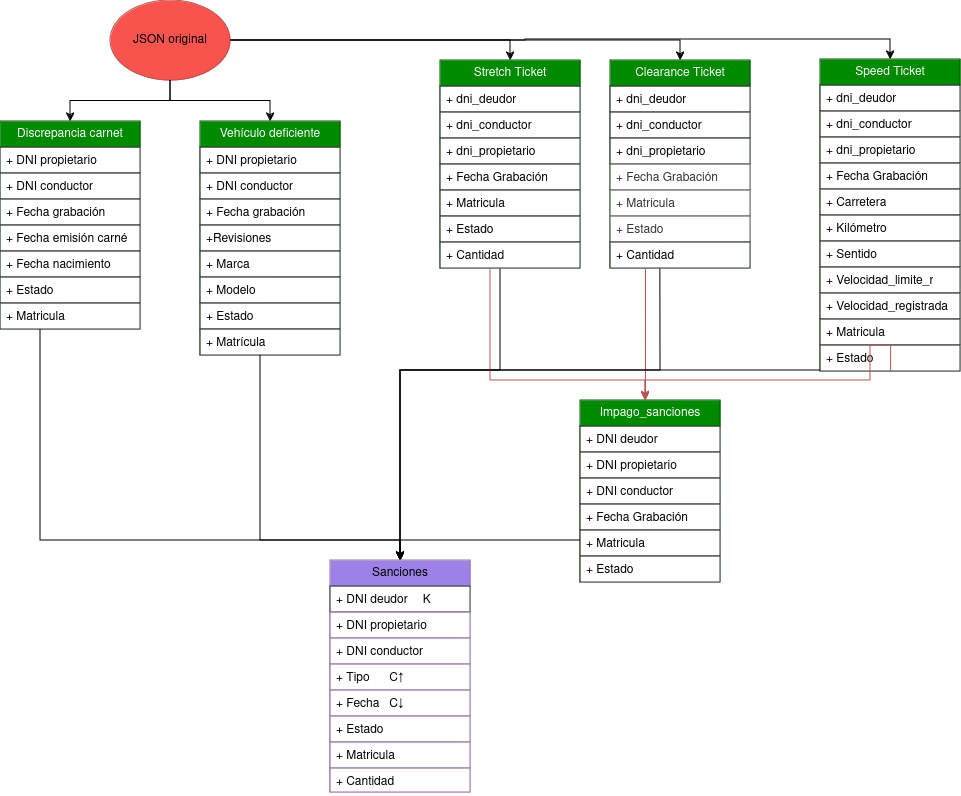
\includegraphics[width=0.8\textwidth]{./imagenes/Sanciones.png}
    \caption{Modelo lógico de Sanciones}
    \label{fig:modelo_sanciones}
\end{figure}

En verde se representan los \textit{dataframes} auxiliares que se construyen en \textit{Pyspark}.


\newpage
\section{Conclusión}
\label{sec:conclusion}

\end{document}
